% 当前 IIoT 数据主稿的中文对照版；C1 窗口与完整 C2/C3 工作负载。
% 以英文稿 main.tex 为准逐段对应：段落切分、编号、公式、算法、表格与引用标签完全一致。
% 保留 pdfLaTeX 与 XeTeX 下一致的 Times 字形度量。
\RequirePackage[OT1]{fontenc}
\documentclass[10pt,journal]{IEEEtran}
\usepackage{graphicx,amsmath,amssymb,booktabs,array,url}
\usepackage{fontspec,xeCJK}
% Windows CJK fonts verified with the desktop editor compiler (XeLaTeX).
\setmainfont{TeX Gyre Termes}
\setCJKmainfont{SimSun}[BoldFont=SimHei,ItalicFont=KaiTi,BoldItalicFont=KaiTi]
\setCJKsansfont{SimHei}
\setCJKmonofont{FangSong}
\renewcommand{\abstractname}{摘要}
\renewcommand{\IEEEkeywordsname}{关键词}
\renewcommand{\figurename}{图}
\renewcommand{\tablename}{表}
\renewcommand{\refname}{参考文献}
\linespread{1.10}
\usepackage[nocompress]{cite}
\interdisplaylinepenalty=2500
\usepackage[colorlinks=true,allcolors=blue]{hyperref}

\newcounter{algorithm}
\renewcommand{\thealgorithm}{\arabic{algorithm}}
\makeatletter
\newcommand{\fps@algorithm}{tbp}
\newcommand{\ftype@algorithm}{1}
\newcommand{\ext@algorithm}{loa}
\newcommand{\fnum@algorithm}{算法~\thealgorithm}
% Local ruled algorithm caption; leave IEEE table/figure captions untouched.
\newenvironment{algorithm}[1][t]{\@float{algorithm}[#1]%
  \long\def\@makecaption##1##2{%
    \par\hrule height .8pt\kern2pt
    {\normalfont\normalsize\noindent\textbf{##1:} ##2\par}%
    \kern2pt\hrule height .8pt\kern2pt}%
}{\end@float}
\makeatother
\newcommand{\ARC}{ARC-Audit}
\newcounter{proposition}
\newenvironment{proposition}[1]{%
  \refstepcounter{proposition}\par\smallskip\noindent
  \textbf{命题~\theproposition\ (#1). }\ignorespaces
}{\par\smallskip}
\newenvironment{claimproof}{\par\noindent\emph{证明：}\ignorespaces
}{\hfill\textit{证毕。}\par\smallskip}
\newcounter{algline}
\newcommand{\al}{\stepcounter{algline}\thealgline:}
\newcommand{\tabnote}[1]{\par\smallskip\parbox{\linewidth}{\footnotesize #1}}
\title{ARC-Audit：面向工业物联网数据的\\依赖感知审计与认证记录恢复}
\author{匿名作者}
\begin{document}
\bstctlcite{IEEEexample:BSTcontrol}
\maketitle
\begin{abstract}
共享压缩可降低工业物联网（Industrial Internet of Things，IIoT）数据的存储开销，但也将单条记录的解码与共享字典页耦合起来。加密隐藏了记录所引用的具体字典行，因此没有解密密钥的公开验证者与持有密钥的授权恢复者需要覆盖不同的页集合。ARC-Audit 通过单一认证布局将逻辑比特区间映射到密文页，从而解决这一信息不对称问题。公开验证者利用该布局构造覆盖所有潜在解码依赖的认证恢复闭包（authenticated recovery closure，ARC），合并目标记录之间的重叠页，并发起新鲜聚合挑战。相比之下，授权恢复者先认证并解密引用页以定位确切字典行，再获取其余依赖页。在每批次存储预算内，ARC-Audit 对选定密文页实施擦除编码保护，并对直接获取与经修复得到的对象执行相同的完整性检查。本文分析解码正确性、闭包覆盖范围、等泄漏条件下的内容保密性，以及聚合响应与返回记录的真实性。在 HAI 数据集的两个数据段上，分组共享表示以更长的构建时间为代价降低了安全云端存储开销，而聚合审计在相同闭包上以更多本地处理换取较低的应用层流量。在固定字典页优先保护且名义擦除率为 5\% 时，相较于获取完整公开闭包，按实际依赖取页使两个数据段的完整记录恢复率分别从 10.8\% 提高到 14.8\%、从 18.0\% 提高到 21.6\%。
\end{abstract}
\begin{IEEEkeywords}
工业物联网，广义去重，公开完整性审计，认证记录恢复，依赖闭包，认证加密。
\end{IEEEkeywords}

\section{引言}\label{sec:introduction}
外包存储的工业物联网（Industrial Internet of Things，IIoT）归档既要支持公开完整性审计，也要能可靠地恢复目标记录。共享压缩利用传感器字段与记录之间的重复结构来节省存储空间。例如，广义去重（generalized deduplication，GD）将数据块表示为共享基及记录特有的引用与偏差~\cite{Talasila2019}，基于相似性的安全去重也已应用于外包 IIoT 存储~\cite{Gao2024}。然而，共享引入了跨对象解码依赖：重建一条记录需要同时取得记录专属对象与共享字典页，且所有对象均须针对所请求的数据版本完成认证。

当字典引用以密文形式存储时，公开验证者与授权恢复者面临天然的信息不对称，因而会为同一记录选出不同的页集合。由于缺乏解密密钥，公开验证者只能依赖认证布局，必须将相关组的完整字典纳入审计范围，以覆盖所有可能被引用的行。授权恢复者则可先解密引用，仅获取实际指明的字典页。因此，即使某个未被引用的字典页丢失而导致完整公开闭包无法取得，目标记录本身仍可能正常解码。

现有研究各自优化上述流程的某一环节：压缩方法改进数据表示~\cite{Hurst2024GreedyGD}，公开存储证明验证受挑战对象的响应~\cite{ShachamWaters2013}，选择性访问系统优化查询取数~\cite{Taurone2024TREAT}，共享存储保护则缓解公共块丢失带来的影响~\cite{Bhagwat2006Reliability}。连接这些问题的核心在于：在各角色可获得的信息下确定哪些密文页足以解码请求记录，并将这些页绑定到同一认证版本。

ARC-Audit 引入\emph{认证恢复闭包}（authenticated recovery closure，ARC），在同一份压缩批次上统一两类角色的依赖选取。数据所有者发布已签名布局，将逻辑比特区间映射到密文页，同时将完整解码内容保留为密文。公开验证者据此收集相关组字典，合并多目标之间的重叠页，并将所得闭包绑定至新鲜聚合挑战。授权恢复者先认证并解密引用页以解析实际依赖，再获取其余对象。在每批次存储预算内，ARC-Audit 对选定密文页施加 Reed--Solomon（RS）编码保护，按相同的完整性规则校验修复页与直接获取页，仅在完成确定性完整解码后接受记录。

本文的主要贡献概括如下。
\begin{itemize}
\item \emph{加密布局上的双角色依赖规划。}本文设计了单一认证布局，将结构化的比特区间几何与加密的解码数值分离。这使得公开验证者无需解密密钥即可构造充分闭包，同时允许授权恢复者在认证引用后将取数范围缩减至精确依赖。
\item \emph{依赖感知的公开聚合审计。}我们将闭包规划与基于 BLS12-381 的线性同态认证器结合，合并跨目标重叠页并将快照、目标与所选页集绑定至新鲜挑战，从而避免引用传输与逐页证明开销。
\item \emph{可寻址共享表示与受预算约束的精确恢复。}ARC-Audit 的分组广义去重编码器（SDA-GGD）按全量输入序列化成本确认字段合并，并保留页级区间边界。在擦除恢复方面，密文 RS 层在序列化存储上限内保护选定页，并以与直接取页相同的校验规则验证修复页。
\end{itemize}

本文在 HAI 工业控制数据集的两个数据段上评估 ARC-Audit。字段分组相较按字段独立 GD 降低了安全云端存储开销，但增加了构建时间。审计实验中，公开聚合以更高的本地密码学计算代价换取更低的应用层流量，并省去了授权检索所需的引用传输。在名义擦除率为 5\% 且固定字典页优先保护的条件下，精确依赖解析使部分请求在未引用字典页不可用时仍能完成恢复。
\section{相关工作}
\subsection{共享压缩与选择性访问}
共享压缩在局部编码与共享字典之间划分记录内容。GD 由共享基和逐记录偏差重建数据块~\cite{Talasila2019}。在此基础上，GreedyGD 选择基比特以同时支持压缩与直接分析~\cite{Hurst2024GreedyGD}，EntroGD 则将分析摘要与熵引导压缩相结合~\cite{Zhao2026EntroGD}。上述方案聚焦于压缩率与原位分析，而 ARC-Audit 通过认证记录区间和字典布局将共享表示与密码学验证连接起来，使验证者无需读取引用即可选取密文页。

保密性与选择性访问对共享表示提出了进一步约束。基于相似性的安全去重通过带所有权证明的模糊消息锁定加密~\cite{Jiang2023FuzzyDedup}与外包 IIoT 存储管理~\cite{Gao2024}解决所有权与保密问题。与本文访问模型更接近的是 TREAT~\cite{Taurone2024TREAT}，其结合 GD、编码、重排与选择性获取以支持分布式物联网查询；其 GD 表示支持按 BaseID 寻址字典项，实测查询流程则预先获取完整字典并用 BaseID 做谓词过滤。相比之下，ARC-Audit 在同一认证布局上服务两类角色：公开验证者在引用保持加密时覆盖所有潜在解码依赖，授权恢复者则在接受规范化记录前依次认证引用及其指向的密文依赖。

\subsection{公开审计与可取回性}
公开存储验证针对受挑战对象建立完整性保证。可证明数据持有（PDP）验证外包存储持有性~\cite{Ateniese2007PDP}，可取回性证明（PoR）则通过提取算法将挑战响应与数据恢复关联起来~\cite{Juels2007POR,ShachamWaters2013}。后续研究扩展了 PoR 框架~\cite{Bowers2009PORTheory}，在 HAIL 中将完整性检查与分布式冗余结合~\cite{Bowers2009HAIL}，并在动态 PDP 中利用认证字典支持更新~\cite{Erway2009DPDP}。近期的压缩 PDP 构造进一步降低了认证器存储开销，并通过线性通信的证明交换实现去中心化多云自审计~\cite{Yang2025CompressedPDP}。与挑战任意分块或整份文件不同，ARC-Audit 直接依据记录的解码依赖推导待挑战页集合。

共享数据审计同样致力于降低认证冗余并支持选择性验证。早期方案通过带去重的存储证明~\cite{Zheng2012POSD}、共享认证器~\cite{Tian2022SharedAudit}、客户端链下去重~\cite{Zhang2023BlockchainAudit}以及削减密钥与认证器冗余~\cite{Miao2024SharedAudit}来融合审计与去重。隐私保护变体在加密去重与审计中保护文件所有权~\cite{Song2023EncryptedAudit}，或结合基于身份的广播加密密钥管理来保护文件标签与审计证明隐私~\cite{Zhang2025PrivacyAudit}。细粒度去重进一步衔接了审计与数据取回：Liu 等对用户内及跨用户的密文与认证标签去重，并借助重构矩阵与 Bloom 过滤器取回分布式去重块~\cite{Liu2025FineGrained}；带仲裁的可搜索审计~\cite{Miao2025}、动态混合审计~\cite{Pan2026}及可更新多副本认证~\cite{Xu2026MPA}则分别解决其他共享存储场景下的选择性验证问题。

认证数据结构将目录查询应答绑定至数据源认证的承诺~\cite{Goodrich2003ADS}。ARC-Audit 将这一原则延伸至共享压缩记录的解码过程：公开验证者在选取充分闭包前验证签名布局，授权恢复者则在通过 BaseID 解析字典行前认证引用页。

\subsection{共享存储可靠性}
保护共享存储必须计入每项对象所服务的记录，因为公共块丢失会波及多条逻辑记录。已有研究通过基于丢失影响的复制~\cite{Bhagwat2006Reliability}及去重擦除编码存储的可靠性分析~\cite{Li2010Reliability}阐明了这种依赖效应。在系统层面，CDStore 将收敛分散与两阶段去重相结合，以协同多云环境下的可靠性、安全性与存储效率~\cite{Li2015CDStore}；Per-File Parity 将去重前校验与文件内、文件间恢复相结合~\cite{Wu2019PFP}；RepEC+ 则协同组织复制、擦除编码、对象选择与协同恢复~\cite{Zuo2022RepECPlus}。ARC-Audit 对完整密文页应用标准 RS 编码~\cite{ReedSolomon1960}，在固定编码参数与存储预算下评估保护位置部署和精确依赖选择对认证记录恢复的影响。

\section{系统模型与问题定义}\label{sec:model}
给定一个不可变批次快照和目标记录集合 $T$，ARC-Audit 在同一份压缩数据上支持公开审计与授权恢复。记录可以引用共享字典中的条目，而具体引用保存在加密页中。公开验证者需要从认证布局确定审计范围。授权恢复者可以解密引用，确定实际参与解码的页。两条路径由此得到各自所需的页集合。

\subsection{系统角色与可信状态}
图~\ref{fig:architecture}~展示了四类角色。\emph{数据所有者}独立编码并加密每个批次，生成公开审计标签，签署批次清单，并在本地保留批次级共享基目录与私有编码状态。\emph{云服务提供商}（cloud service provider，CSP）存储密文页、审计标签、公开参数、签名布局及已部署的辅助保护文件，负责生成审计响应并提供请求的对象。

\emph{公开验证者}在发起挑战前认证布局和审计参数。\emph{授权恢复者}还持有批次解密能力，可用经过认证的对象恢复记录。两类客户端均以所有者的验证公钥和预期清单摘要为可信锚点。签名清单绑定批次标识、布局、页的身份、长度与摘要、协议和审计参数。快照是该清单承诺的不可变编码状态。客户端保留完整的认证清单，因此其元数据开销随页数增长。加密、清单签名和审计标签使用独立的秘密材料。跨批次请求按批次处理，各自使用对应的可信锚点与密码上下文。

\subsection{记录与页依赖}
在声明模式下，规范化记录包含经缩放的过程值、索引、时间和标签。对批次 $b$，逻辑编码容器 $F$ 被划分为至多 $P_0$ 字节的明文切片 $F_p$。\emph{页}指一个切片对应的完整密文对象 $C_p$，由批次标识和局部页索引 $(b,p)$ 唯一标识。令 $\mathcal P$ 为所有此类页标识的集合，$\mathcal L$ 为经过认证的公开布局。布局将逻辑比特区间 $[a,a+w)$ 映射到它跨越的所有页：
\begin{equation}\label{eq:phi}
\Phi_{\mathcal L}(a,w)=
\left\{(b,p):\left\lfloor\frac{a}{8P_0}\right\rfloor
\leq p\leq\left\lfloor\frac{a+w-1}{8P_0}\right\rfloor\right\},
\end{equation}
其中 $\Phi_{\mathcal L}(a,0)=\varnothing$。

对给定的编码表示和确定性解码器，精确依赖集 $\mathcal D_{\mathcal L}(i)$ 包含解码记录 $i$ 实际使用的结构、引用、局部数据、标签和所引用字典行所在的页。公开恢复闭包 $K_{\mathcal L}(i)$ 将相关组的完整字典纳入范围，以覆盖所有可能的引用所需的解码输入：
\begin{equation}\label{eq:sufficient-set}
\mathcal D_{\mathcal L}(i)\subseteq K_{\mathcal L}(i)\subseteq\mathcal P.
\end{equation}
对请求 $T$，令 $U(T)=\bigcup_{i\in T}K_{\mathcal L}(i)$ 为公开闭包并集，$D(T)=\bigcup_{i\in T}\mathcal D_{\mathcal L}(i)$ 为精确依赖并集，因此 $D(T)\subseteq U(T)$。验证者从布局计算 $U(T)$。恢复者先认证并解密引用页，再确定 $D(T)$。

\subsection{威胁模型与公开视图}
模型假设所有者诚实构建批次，客户端使用真实的可信锚点和预置密钥执行协议。不可信 CSP 可以观察公开状态和请求，也可以遗漏对象、修改密文、替换元数据或标签，以及重放快照或响应。预期清单摘要固定本次请求的快照，新鲜挑战将响应与当前审计上下文绑定。清单认证依赖签名的不可伪造性和哈希的抗碰撞性。

公开视图包括记录数量、页长度、关联数据、组与比特结构、字典基数、可见的保护布局，以及公开审计请求的目标和页集合。常量、时间与标签内容、引用、共享基和偏差等私有解码值均加密存储。若部署中可观察授权恢复的取页轨迹，由于该轨迹可能随私有引用变化，也应纳入泄露定义。第~\ref{sec:security}~节针对泄露相同的输入定义内容保密性，并给出密钥派生与带关联数据的认证加密（AEAD）假设。

\subsection{审计、恢复与保护目标}
\emph{公开审计。} 对目标集合 $T$，验证者认证签名元数据，并向 CSP 发起覆盖 $U(T)$ 的挑战。只有所有涉及批次的聚合响应均在预期挑战上下文中通过验证，审计才接受。该真实性目标针对指定快照上所选页的聚合响应。

\emph{授权恢复。} 令 $\mathcal A$ 为恢复者已取得承诺密文并通过明文认证的页集合，其中的页可直接获取或经验证的擦除修复获得。设 $\widehat r_i$ 为解码结果，$r_i$ 为原始规范化记录，记录 $i$ 的恢复成功条件定义为
\begin{equation}\label{eq:record-recovery}
\mathsf{Rec}_i(\mathcal A)=
\mathbf1\{\mathcal D_{\mathcal L}(i)\subseteq\mathcal A
\ \land\ \widehat r_i=r_i\}.
\end{equation}
运行时，恢复者验证所需输入的真实性并检查能否完整解码，返回全部请求的规范化记录或报告失败。第~\ref{sec:security}~节给出依赖绑定、精确解码和返回记录真实性的成立条件。

\emph{预算内保护。} 同一页可能被多条记录依赖，因此保护哪些页会影响页缺失后哪些记录仍可恢复。保护层以每批次密文存储量的比例 $\beta$ 为辅助存储上限，在预算内分配冗余以提高记录恢复机会。第~\ref{sec:protection}~节给出计费口径和不同的分配策略，第~\ref{sec:eval}~节比较这些策略。

\begin{table}[t]\centering\small
\caption{ARC-Audit 的符号说明}\label{tab:notation}
\begin{tabular}{@{}l>{\raggedright\arraybackslash}p{.70\columnwidth}@{}}\toprule
符号 & 含义\\\midrule
$b$, $b_T$ & 批次标识；$T$ 涉及的批次数\\
$F,F_p,C_p$ & 逻辑容器、明文切片、密文对象\\
$k_b,N_p,A_p$ & 批次加密密钥、nonce、关联数据\\
$\mathcal L,\Phi_{\mathcal L}$ & 认证公开布局与比特区间映射\\
$\ell(p),\tau_p$ & 密文有效长度与公开审计标签\\
$\mathcal D(i),K(i)$ & 精确依赖与公开充分闭包\\
$D(T),U(T)$ & 精确依赖并集与审计闭包并集\\
$\pi=(\sigma,\boldsymbol\mu)$ & 聚合审计响应\\
$\beta,B_{\rm side}$ & 保护预算比例与计费辅助保护文件字节数\\\bottomrule
\end{tabular}\end{table}

\begin{figure*}[t]\centering
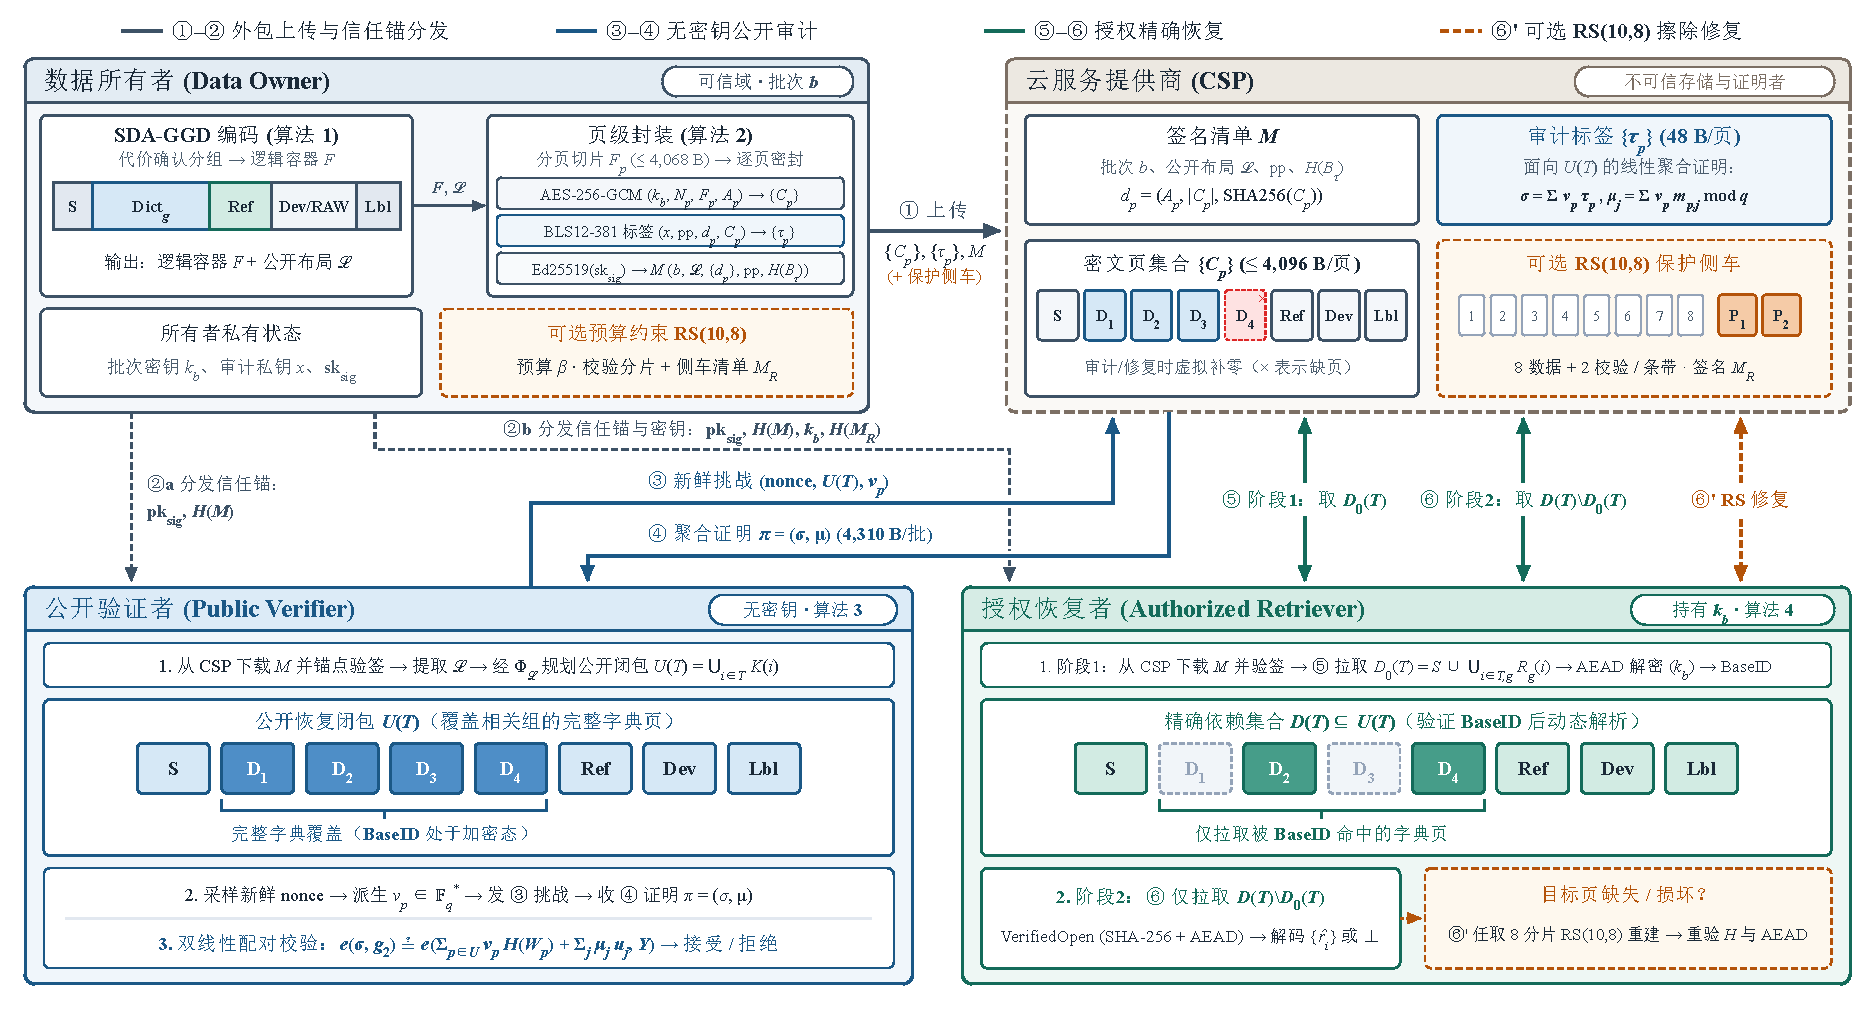
\includegraphics[width=\textwidth]{figures/cn/architecture.pdf}
\caption{ARC-Audit 的系统架构。图中的页块示意公开审计与授权恢复各自覆盖的字典页。}
\label{fig:architecture}\end{figure*}

\section{ARC-Audit 方案设计}\label{sec:design}
\subsection{方案概述}
图~\ref{fig:architecture}~展示了公开审计与授权恢复如何从同一批次中选取密文页。数据所有者用 SDA-GGD 对记录进行分组编码，将逻辑容器封装为可寻址的密文页，并在签名清单中承诺其布局。两类客户端均依据预置可信锚点认证布局。公开验证者将相关组的全部字典页纳入充分闭包，合并各目标记录的闭包得到 $U(T)$，随后发起新鲜挑战并验证 CSP 的聚合响应。授权恢复者先认证解密引用页并读取 BaseID，根据这些引用指向的字典行确定精确依赖集合 $D(T)$，再获取其余页，在验证全部必需输入后解码规范化记录。

保护层在存储预算内为选定密文对象部署冗余，并通过原有的认证获取接口提供修复页。

\subsection{经全量成本确认的共享表示}\label{sec:c1}
ARC-Audit 使用 SDA-GGD 对字段分组，在减少编码字节数的同时保留定位依赖所需的信息。编码器按样本收益对候选合并排序，再根据全量输入的序列化成本决定是否接受合并。所得布局标明记录区间与字典范围，使验证者在读取引用前即可选取审计所需的页。

\emph{编码与序列化成本。}在声明模式下，每个字段被赋予精确的十进制缩放与整数位宽。常量只存储一次，其余字段被划分为若干组。对于总位宽为 $L_g$ 的组 $G$，编码器选择 $k$ 个基比特位置；令 $M_g$ 表示观测到的不同共享基数量。其余 $L_g-k$ 个位置构成偏差。每条记录在其偏差之外存储长度为 $b_g=\lceil\log_2 M_g\rceil$ 比特的定宽共享基标识，组字典则存储共享基。对于 $n$ 条记录，组的序列化成本为
\begin{equation}\label{eq:cost}
\begin{split}
C(G)={}&C_{\mathrm{hdr}}(G,k)+\lceil M_gk/8\rceil+\lceil nb_g/8\rceil\\
 &+\lceil n(L_g-k)/8\rceil,
\end{split}
\end{equation}
其中 $C_{\mathrm{hdr}}(G,k)=11+2|G|+2k$ 字节用于存储组模式、字段标识和基比特位置。RAW 组的成本为 $C_{\mathrm{hdr}}(G,0)+\lceil nL_g/8\rceil$。各数据流独立进行字节取整，因为这些流分别序列化。完整容器的成本为 $C_0+\sum_G C(G)$，其中 $C_0$ 包含固定模式、常量、时间／标签表示和全局头部。

\emph{组内配置。}$\operatorname{Config}(X,G)$ 按经验二元熵递增对组内比特位置进行稳定排序，依次测试长度为 $k=0,1,\ldots,L_g$ 的前缀。当 $M_g=n$ 时停止。对合并组，熵相同时保留字段拼接后的局部比特顺序。对每个前缀，令 $n_b$ 为共享基 $b$ 的记录数。当前缀的 $R_{\mathrm{dep}}=\max_b n_b/n\leq\rho$ 时，该前缀可行。配置器在可行前缀中选择式~\eqref{eq:cost}~所给序列化成本最低者，成本相同时取较小的 $k$。若没有可行前缀，则依次按 $R_{\mathrm{dep}}$、成本和 $k$ 从小到大选择。若 RAW 成本不高于所选 GD 配置，则返回 RAW。

\emph{样本排序与全量确认。}初始化时每个非常量字段构成一个活动组。固定样本给出联合字节收益 $\widehat\Delta=C_m(G_a)+C_m(G_b)-C_m(G_a\mathbin{\|}G_b)$，其中 $C_m$ 在相同样本行上配置并测量各组，$\|$ 表示有序字段拼接。只有样本收益为正的组对才进入队列。在全量确认前，算法先刷新候选收益并剔除过期版本。在合并 $G_a$ 与 $G_b$ 之前，编码器在全部输入记录上重新配置组合组并计算
\begin{equation}
\Delta_{\mathrm{full}}=C(G_a)+C(G_b)-C(G_a\mathbin{\|}G_b).
\end{equation}
合并须同时满足全量序列化字节收益与载荷收益为正，随后更新受影响的候选，直至队列为空。RAW 回退计入配置的真实字节成本。算法~\ref{alg:grouping}~以精确记录 $X$、模式 $\Sigma$ 和固定样本索引 $I$ 为输入。辅助函数 $\operatorname{Config}(X,G)$ 选择含 RAW 回退在内的组配置；$C(G;c)$ 和 $C_{\mathrm{pay}}(G;c)$ 分别表示配置 $c$ 下的序列化成本及不含组头部的字节取整载荷成本（省略 $c$ 时指当前配置）。$\operatorname{SampleGain}$ 返回样本收益与合并配置，但仅凭样本估计不能授权合并。

由于合并两个组会改变相邻组对的收益，算法~\ref{alg:grouping}~在 $J$ 中记录已拒绝的带版本组对，并丢弃端点版本已过期的条目。为防止刷新后收益下降的候选阻塞队列或无限循环，$\operatorname{TopGain}$ 返回队列头部存储的收益（空队列返回 $-\infty$），相同优先级按入队顺序处理，且每个候选在全量输入检验前最多延后 $d_{\max}=8$ 次（由 $d_e$ 计数）。

\begin{algorithm}[t]\centering\normalsize\setcounter{algline}{0}
\caption{全量成本确认分组}\label{alg:grouping}
\begin{tabular}{@{}r@{\enspace} >{\raggedright\arraybackslash}p{.88\columnwidth}@{}}
\multicolumn{2}{@{}p{\columnwidth}@{}}{\textbf{输入：}记录 $X$，模式 $\Sigma$，样本索引 $I$。}\\
\multicolumn{2}{@{}p{\columnwidth}@{}}{\textbf{输出：}逻辑容器 $F$ 与公开布局 $\mathcal L$。}\\
\al & $\mathcal G\gets$ 每个非常量字段构成一个组。\\
\al & 在 $X$ 与 $X_I$ 上配置 $\mathcal G$；$J\gets\varnothing$。\\
\al & $Q\gets$ 样本收益为正的组对；初始化 $d_e=0$。\\
\al & \textbf{当} $Q\neq\varnothing$ \textbf{时执行}\\
\al & \hspace*{1em}$e=(G_a,G_b,\text{versions})\gets\operatorname{PopMax}(Q)$。\\
\al & \hspace*{1em}\textbf{若} $e$ 过期或 $e\in J$，\textbf{继续}。\\
\al & \hspace*{1em}$(\widehat\Delta,\widehat c)\gets\operatorname{SampleGain}(X_I,G_a,G_b)$。\\
\al & \hspace*{1em}\textbf{若} $\widehat\Delta\leq0$，将 $e$ 加入 $J$；\textbf{继续}。\\
\al & \hspace*{1em}\textbf{若} $\operatorname{TopGain}(Q)>\widehat\Delta$ 且 $d_e<d_{\max}$，\textbf{则}\\
\al & \hspace*{2em}$d_e\gets d_e+1$；以 $\widehat\Delta$ 将 $e$ 重新入队；\textbf{继续}。\\
\al & \hspace*{1em}\textbf{结束条件分支}\\
\al & \hspace*{1em}$G_c\gets G_a\mathbin{\|}G_b$；$c\gets\operatorname{Config}(X,G_c)$。\\
\al & \hspace*{1em}$\Delta_{\mathrm{full}}\gets C(G_a)+C(G_b)-C(G_c;c)$。\\
\al & \hspace*{1em}$\Delta_P\gets C_{\mathrm{pay}}(G_a)+C_{\mathrm{pay}}(G_b)-C_{\mathrm{pay}}(G_c;c)$。\\
\al & \hspace*{1em}\textbf{若} $\Delta_{\mathrm{full}}>0$ 且 $\Delta_P>0$，\textbf{则}\\
\al & \hspace*{2em}用带有 $(c,\widehat c)$ 的 $G_c$ 替换 $\mathcal G$ 中的 $G_a,G_b$。\\
\al & \hspace*{2em}使旧组条目失效；将收益为正的新组／存活组对入队。\\
\al & \hspace*{1em}\textbf{否则}将 $e$ 加入 $J$。\\
\al & \hspace*{1em}\textbf{结束条件分支}\\
\al & \textbf{结束循环}\\
\al & $(F,\mathcal L)\gets\operatorname{Serialize}(X,\Sigma,\mathcal G)$。\\
\al & \textbf{返回} $(F,\mathcal L)$。\\\bottomrule
\end{tabular}\end{algorithm}

\begin{proposition}{经确认的逻辑成本下降}\label{prop:cost}
每次被接受的合并都严格降低经检查的逻辑序列化成本及其载荷成本。从 $g_0$ 个活动组出发，至多接受 $g_0-1$ 次合并。
\end{proposition}
\begin{claimproof}
算法~\ref{alg:grouping}~仅在两项收益均为正时接受合并。未参与合并的组及容器固定部分的成本保持不变，因此合并严格降低逻辑序列化成本及其载荷成本。每次合并使活动组数减一，故至多接受 $g_0-1$ 次合并。算法记录已拒绝的带版本组对、丢弃过期条目并限制重新入队次数，因而两次合并之间的候选处理也会终止。
\end{claimproof}
式~\eqref{eq:cloud-cost}~中的实测安全云端成本还包含加密封装、审计标签和公开清单。第~\ref{sec:eval}~节将这一最终成本与逻辑分组目标分别评估。


\subsection{页加密与认证布局}\label{sec:seal}
ARC-Audit 的页加密与认证布局将依赖定位所需的结构信息与私有解码数值分开。公开布局包含流位置、位宽、模式、基比特位置、字典基数与记录数量。该布局支持式~\eqref{eq:phi}~的页映射；私有解码头部与数值（包括数值常量与私有字段值）则与编码记录一起保留在完整逻辑容器的加密切片中。

每次构建时，所有者抽取新的 256 比特批次标识 $b$ 与随机加密主秘密，再以 $b$ 为盐、\texttt{ARC/ENC/v1} 为上下文通过 HKDF-SHA256 派生 $k_b$~\cite{RFC5869}。nonce $N_p$ 为局部页索引的 96 比特编码，同一批次密钥下各页 nonce 互不相同。关联数据 $A_p$ 是协议、所有者域、批次、对象身份、编解码器和明文长度的规范编码，并保留在公开描述符中。每个明文切片至多 $P_0=4,068$ B，AES-256-GCM 按下式封装切片~\cite{RFC5116}：
\begin{equation}\label{eq:cipher}
C_p=N_p\,\|\,\mathsf{Enc}_{k_b}(N_p,F_p,A_p).
\end{equation}
12 字节 nonce 与 16 字节认证标签使密文有效长度为 $\ell(p)=|F_p|+28\leq4,096$ B，末尾切片保留实际长度。大小为 $B_F>0$ 字节的容器共有 $N=\lceil B_F/P_0\rceil$ 页，密文占用 $B_{\rm cipher}=B_F+28N$ 字节，而审计与修复使用的虚拟零填充不占用密文存储空间。

每个描述符还记录完整密文长度与 SHA-256 摘要，对应的审计标签则将该描述符绑定到公开参数指纹。生成全部密文对象与标签之后，所有者按页索引递增顺序序列化标签，并用 Ed25519 签署包含对象描述符、公开布局、审计参数以及标签文件 SHA-256 摘要的规范清单。由此得到的 32 字节清单摘要和 32 字节签名公钥构成客户端预置可信锚点。这一顺序既把标签绑定到不可变密文，又把清单绑定到已完成标签，同时避免了循环摘要依赖（算法~\ref{alg:seal}）。

\begin{algorithm}[t]\centering\normalsize\setcounter{algline}{0}
\caption{封装一个数据批次}\label{alg:seal}
\begin{tabular}{@{}r@{\enspace} >{\raggedright\arraybackslash}p{.88\columnwidth}@{}}
\multicolumn{2}{@{}p{\columnwidth}@{}}{\textbf{输入：}逻辑容器 $F$，公开布局 $\mathcal L$，所有者域。}\\
\multicolumn{2}{@{}p{\columnwidth}@{}}{\textbf{输出：}密文对象、审计标签、签名清单与客户端可信锚点。}\\
\al & 抽取新的批次 $b$ 与加密主秘密；派生 $k_b$。\\
\al & 生成独立的审计秘密 $x$、公开参数 $\mathsf{pp}$ 与清单签名密钥。\\
\al & \textbf{对每个}至多 4,068 B 的切片 $F_p$ \textbf{执行}\\
\al & \hspace*{1em}$N_p\gets\operatorname{Encode}_{96}(p)$；构造关联数据 $A_p$。\\
\al & \hspace*{1em}$C_p\gets N_p\|\mathsf{Enc}_{k_b}(N_p,F_p,A_p)$。\\
\al & \hspace*{1em}$d_p\gets(A_p,|C_p|,\mathsf{Hash}(C_p))$。\\
\al & \hspace*{1em}$\tau_p\gets\operatorname{Tag}(x,\mathsf{pp},d_p,C_p)$。\\
\al & \textbf{结束循环}\\
\al & 按页索引递增顺序序列化标签，得到 $B_\tau$。\\
\al & $M\gets\operatorname{Manifest}(b,\mathcal L,\{d_p\},\mathsf{pp},\mathsf{SHA256}(B_\tau))$。\\
\al & 签署规范清单 $M$；预置签名公钥与 $\mathsf{Hash}(M)$ 作为可信锚点。\\
\al & 保留批次级私有编码状态与解密能力。\\
\al & \textbf{返回} $\{C_p\},\{\tau_p\},M$、签名与可信锚点。\\\bottomrule
\end{tabular}\end{algorithm}

\subsection{认证恢复闭包}\label{sec:c2}
给定目标集合 $T$ 与认证布局 $\mathcal L$，ARC-Audit 的公开闭包规划由布局计算足以覆盖解码依赖的页并集 $U(T)$，其中包含每个相关组的字典。在位区间映射 $\Phi_{\mathcal L}$ 下，令 $S$ 表示覆盖私有结构元数据的页，$R_g(i)$ 表示记录 $i$ 在组 $g$ 中引用区间所覆盖的页，$V_g(i)$ 表示其偏差或 RAW 内容所覆盖的页，$L(i)$ 表示其标签所覆盖的页。令 $\mathcal P_g^{\rm dict}$ 包含 GD 组映射后的全部字典页。单记录公开恢复闭包定义为
\begin{equation}\label{eq:closure}
K(i)=S\cup L(i)\cup\bigcup_g
\bigl(R_g(i)\cup V_g(i)\cup\mathcal P_g^{\rm dict}\bigr).
\end{equation}
RAW 组没有引用和字典，因此相应的集合为空。私有结构包含解码所需的模式与格式信息；标签项覆盖目标记录的标签比特。凡是与所选区间相交的密文页均会纳入，即使同一页还包含其他逻辑流的数据。

公开验证者依据认证布局构造 $K(i)$，用完整组字典覆盖任意有效 BaseID 所选中的行。授权恢复者则认证并解密 $S$ 与引用页，在承诺位置读取各 BaseID、检查其范围，并映射被引用的字典行。把这些字典行页与 $S$、引用、局部内容和标签合并，即得到精确依赖集 $\mathcal D(i)$。

对于目标集合 $T$，公开请求把重叠的单记录闭包合并为 $U(T)=\bigcup_{i\in T}K(i)$。给定密文长度 $\ell(p)$，并集规划与不带缓存的分别遍历所读取的逻辑字节数为
\begin{equation}\label{eq:reads}
B_U=\sum_{p\in U(T)}\ell(p),\qquad
B_N=\sum_{i\in T}\sum_{p\in K(i)}\ell(p).
\end{equation}
在同一次请求中，缓存也能让逐记录遍历只读取每个对象一次。实验分别比较缓存或并集规划带来的读取复用，以及聚合证明带来的认证开销变化。当请求涉及多个批次时，先按批次计算目标及其对象并集，再以带批次标识的对象身份汇总请求。

\subsection{基于新鲜挑战的公开聚合审计}\label{sec:audit}
ARC-Audit 的 Public-Aggregate 接口验证公开闭包上的线性响应。验证者将目标记录、快照和所选对象纳入每次新生成的挑战，使响应与当前请求及所指定的数据版本绑定。

每个完整密文对象被编码为 $s=133$ 个 31 B 的小端扇区，并在其有效长度之外进行虚拟零填充。对于 BLS12-381 的标量阶 $q$，扇区整数满足 $m_{p,j}<2^{248}<q$。因此该扇区化覆盖 nonce、加密载荷与 AEAD 标签；签名有效长度决定尾部去除。

沿用 Shacham--Waters 线性公开认证结构~\cite{ShachamWaters2013}，所有者选择秘密 $x$，公开 $Y=xg_2$，并在配对 $e:\mathbb G_1\times\mathbb G_2\to\mathbb G_T$ 下在 $\mathbb G_1$ 中计算标签：
\begin{equation}\label{eq:tag}
\tau_p=x\left(H(W_p)+\sum_{j=1}^{s}m_{p,j}u_j\right).
\end{equation}
$W_p$ 绑定完整密文描述符与参数指纹。基点 $u_j$ 与描述符哈希 $H$ 使用域分离的哈希到曲线运算~\cite{RFC9380}。

对每个批次请求，验证者生成新的 256 比特 nonce。规范挑战绑定快照、公开参数、目标集合、所选页集合、请求策略与会话。非零系数 $\nu_p$ 由该完整上下文派生。以规范挑战的摘要、页索引和重试计数器作为 SHA-512 的输入，将输出对 $q$ 取模，若为零则递增计数器重试，得到 $\nu_p\in\mathbb F_q^*$。收到挑战后，CSP 读取每个所选页并返回
\begin{equation}\label{eq:aggregate}
\sigma=\sum_{p\in U}\nu_p\tau_p,\qquad
\mu_j=\sum_{p\in U}\nu_pm_{p,j}\pmod q.
\end{equation}
在完成上下文、格式、曲线点、子群、标量范围与维度检查之后，验证者检验
\begin{equation}\label{eq:pairing}
e(\sigma,g_2)=e\left(\sum_{p\in U}\nu_pH(W_p)+\sum_j\mu_ju_j,Y\right).
\end{equation}
验证者以自己计算的页集合为准。公开参数排除无效基点与单位元，响应须同时通过解析检查和式~\eqref{eq:pairing}~的配对验证。算法~\ref{alg:audit}~给出公开审计流程。

\begin{algorithm}[t]\centering\normalsize\setcounter{algline}{0}
\caption{ARC-Audit 的公开闭包审计}\label{alg:audit}
\begin{tabular}{@{}r@{\enspace} >{\raggedright\arraybackslash}p{.88\columnwidth}@{}}
\multicolumn{2}{@{}p{\columnwidth}@{}}{\textbf{输入：}目标 $T$、对应的清单与可信锚点、公开审计参数。}\\
\multicolumn{2}{@{}p{\columnwidth}@{}}{\textbf{输出：}\texttt{ACCEPT} 或 \texttt{REJECT}。}\\
\al & 若 $T$ 为空则拒绝。按不可变批次划分 $T$。\\
\al & \textbf{对每个}涉及的批次 $b$ \textbf{执行}\\
\al & \hspace*{1em}依据可信锚点认证清单，检查 $T_b$ 中的目标是否互异且在有效范围内，并验证公开参数。\\
\al & \hspace*{1em}\textbf{若}验证失败，\textbf{返回} \texttt{REJECT}。\\
\al & \hspace*{1em}$U_b\gets\operatorname{SortUnique}(\bigcup_{i\in T_b}K_{\mathcal L_b}(i))$。\\
\al & \hspace*{1em}抽取新 nonce；绑定预期快照、请求、$T_b$ 与 $U_b$。\\
\al & \hspace*{1em}对 $p\in U_b$ 派生 $\nu_p\in\mathbb F_q^*$；发送挑战并保留预期上下文。\\
\al & \hspace*{1em}CSP 读取唯一的 $C_p$，并用 $p\in U_b$ 的 $\tau_p$ 按式~\eqref{eq:aggregate}~响应。\\
\al & \hspace*{1em}验证者检查格式、上下文、编码与式~\eqref{eq:pairing}。\\
\al & \hspace*{1em}\textbf{若}响应缺失或任一检查失败，\textbf{返回} \texttt{REJECT}。\\
\al & \textbf{结束循环}\\
\al & \textbf{返回} \texttt{ACCEPT}。\\\bottomrule
\end{tabular}\end{algorithm}

序列化聚合证明每批次占 $4+2+48+133\cdot32=4,310$ B，依次计入协议帧头、扇区数量、聚合群元素和标量向量。因此涉及 $b_T$ 个批次的请求包含 $4,310b_T$ 字节的证明，此外还需计入声明与挑战。第~\ref{sec:eval}~节按实际应用层封装，把这一公开接口与授权引用解析和公开下载进行比较。

对于固定挑战，逐页证明对照为每个 $p$ 返回 $(\nu_p\tau_p,(\nu_pm_{p,j})_j)$，并验证相应的单页方程。因此，聚合响应与逐页响应使用相同的所选页与新鲜系数。逐页证明在 4,310 B 的证明格式上增加 8 字节页标识，$u$ 页的证明共占 $4,318u$ 字节。

\subsection{精确认证记录恢复}\label{sec:c3}
ARC-Audit 的精确恢复策略（Exact）先认证并解析引用，再获取并认证实际依赖页。首先，恢复者验证清单、版本可信锚点以及任何辅助保护文件绑定。在第 1 阶段，它获取解析目标所需的结构与引用密文，检查各对象的身份、长度与承诺摘要，并执行 AEAD 认证解密。只有认证这些明文之后，它才解析私有结构与 BaseID、检查其范围并构造精确依赖。在第 2 阶段，覆盖被引用字典行、偏差、RAW 内容与目标标签的其余页经同一验证路径获取。

请求本地缓存保留经过验证的密文与认证明文，使引用解析阶段获得的内容可在依赖获取阶段复用。私有解码器的格式与认证的公开布局进行一致性检查；每次比特读取都必须落在已验证明文之内。在全部必需输入可用之后，确定性解码器重建每条请求的规范化记录。认证、引用范围、格式或解码失败均返回 $\bot$。算法~\ref{alg:recovery}~针对单个批次；多批次恢复对每个涉及批次执行相同过程。

给定对象身份与认证批次上下文，辅助函数 $\operatorname{VerifiedOpen}$ 直接或通过受保护获取接口取得承诺密文，验证其描述符并执行认证解密。它返回验证通过的明文或 $\bot$，并且只缓存经过验证的密文与认证明文。

\begin{algorithm}[t]\centering\normalsize\setcounter{algline}{0}
\caption{ARC-Audit 的精确认证记录恢复}\label{alg:recovery}
\begin{tabular}{@{}r@{\enspace} >{\raggedright\arraybackslash}p{.88\columnwidth}@{}}
\multicolumn{2}{@{}p{\columnwidth}@{}}{\textbf{输入：}清单与可信锚点、解密能力、目标 $T$、云端获取接口。可选输入为签名辅助保护文件及其预置公钥和摘要。}\\
\multicolumn{2}{@{}p{\columnwidth}@{}}{\textbf{输出：}完整解码记录 $\{\widehat r_i\}_{i\in T}$ 或 $\bot$。}\\
\al & 认证清单并验证 $T$。若提供辅助保护文件，依据其可信锚点认证该文件，并检查它与当前批次快照的绑定。\\
\al & \textbf{若}验证失败，\textbf{返回} $\bot$。\\
\al & $I\gets S\cup\bigcup_{i\in T,g}R_g(i)$；$\mathcal C\gets\varnothing$。\\
\al & \textbf{对每个} $p\in I$ \textbf{执行}\\
\al & \hspace*{1em}$\mathcal C[p]\gets\operatorname{VerifiedOpen}(p)$；失败则\textbf{返回} $\bot$。\\
\al & \textbf{结束循环}\\
\al & 解析已认证的私有结构与 BaseID。\\
\al & \textbf{若}解析失败或任一 BaseID 越界，\textbf{返回} $\bot$。\\
\al & 将目标偏差或 RAW 内容页、标签页及经校验的 BaseID 所指字典行覆盖的页并入 $I$，得到 $D(T)$。\\
\al & \textbf{对每个} $p\in D(T)\setminus\operatorname{dom}(\mathcal C)$ \textbf{执行}\\
\al & \hspace*{1em}$\mathcal C[p]\gets\operatorname{VerifiedOpen}(p)$；失败则\textbf{返回} $\bot$。\\
\al & \textbf{结束循环}\\
\al & 检查私有格式与公开布局是否一致，并从 $\mathcal C$ 解码。\\
\al & \textbf{若}格式不一致或无法完整解码，\textbf{返回} $\bot$。\\
\al & \textbf{返回} $\{\widehat r_i\}_{i\in T}$。\\\bottomrule
\end{tabular}\end{algorithm}

Conservative 对照把第 3 行的 $I$ 替换为 $U(T)$；其后的认证与解码完全相同。因此，只要实际解码输入可用或可修复，即使某个未使用的字典对象不可用，精确恢复仍可进行。

\subsection{受预算约束的密文保护}\label{sec:protection}
一个共享页可能参与多条记录的解码。因此，在存储上限相同的情况下，保护哪些页会影响哪些记录能在擦除后恢复。ARC-Audit 对选定的密文对象部署冗余，并在解码前验证修复结果。

GF$(256)$ 上的系统型 RS$(10,8)$ 辅助保护文件把八个密文对象编入一个条带，每个条带存储两个校验分片，同时保留原始密文对象。不足 4,096 B 的对象以虚拟零填充补齐，不完整条带则使用声明的虚拟零槽位。校验在密文上计算，包含 nonce 与 AEAD 标签字节。签名辅助保护文件绑定父快照、编码维度、条带成员与校验摘要。

在分数存储预算 $\beta$ 下，本文为 ARC-Audit 的恢复流程评估三种保护排序。Dictionary 把含字典的页排在其他对象之前，Uniform 使用带种子的置换，FrequencyD 按对象在参考记录集合中的依赖频次排序。三种排序使用共同的条带数量，其取值使每个序列化辅助保护文件都符合相同的每批次上限：
\begin{equation}\label{eq:budget}
B_{\rm side,b}\leq\left\lfloor\beta B_{\rm cipher,b}\right\rfloor.
\end{equation}
每个准入条带存储两个 4,096 字节的校验分片。对于 $s_R$ 个条带及序列化辅助清单 $M_R$，计费总量为 $8,192s_R+|M_R|+128$ 字节，其中 128 字节对应签名、签名公钥和摘要锚点。条带准入以三种排序中的最高计费量为准。实验取 $\beta=0.10$，并以 NoEC 作为零冗余对照。

受保护获取首先检查原始对象。若其不可用，恢复者按承诺摘要验证同一条带中可取得的原始分片与校验分片，并计入签名保护布局声明的虚拟零槽位。通过认证的分片及声明的虚拟零槽位合计达到八个互异槽位时，即可进行 RS 重建。每个重建的真实对象被截断至其签名长度，并在进入缓存之前与其原始密文摘要核对。随后先进行 AEAD 认证，再进行记录解码。同一辅助函数处理引用解析阶段与最终精确依赖集获取阶段所需的修复。

\subsection{计算与存储核算}\label{sec:accounting}
令 $N$ 为批次内的密文对象数，$u=|U(T)|$。除常驻认证元数据之外，直接闭包枚举需要期望 $O(\sum_{i\in T}|K(i)|)$ 的集合插入工作与 $O(u)$ 的唯一对象状态。分组成本对实际执行的样本配置、全量配置与队列更新求和。每次被接受的合并都减少活动组数量。

标签生成处理 $Ns$ 个扇区。生成证明时，服务器累加 $us$ 个域乘积与 $u$ 个加权标签。验证者计算 $u$ 个描述符哈希项和 $s$ 个扇区基点项，再执行两次配对。请求成本按涉及批次累加。每批次的证明大小固定，挑战材料的大小取决于所选页集合，清单大小则随 $N$ 增长。

对于不含辅助保护文件的编码数据，安全云端字节数为
\begin{equation}\label{eq:cloud-cost}
B_{\rm cloud}=B_{\rm cipher}+B_{\rm tags}+B_{\rm manifest},
\end{equation}
其中 $B_{\rm tags}=48N$，签名清单包含公开参数。AEAD 在 $B_{\rm cipher}$ 中贡献 $28N$ 字节。所有者侧共享基字节与总私有状态另行统计。部署辅助保护文件会增加其云端文件；保护状态核算还计入其预置可信锚点。由此区分存储的云端字节与客户端预置状态。

应用层流量计入声明、挑战、响应，以及接口需要时传输的第一阶段引用材料。密文页消息除密文内容外，还包含共 8 字节的帧头与计数，以及每页共 12 字节的标识与长度字段。请求开始计时前，上下文初始化已完成清单与参数的认证和解析。恢复耗时包括获取或修复、认证、解密与解码。修复一个返回页可能需要读取多个分片，因此服务器读取量与应用层回复大小分别统计。

\section{安全性与可恢复性分析}\label{sec:security}
原始依赖页足以解码记录，且公开闭包覆盖这些依赖，这是后续分析的起点。在第~\ref{sec:model}~节的系统模型下，本节依次分析返回记录的真实性、相同公开泄漏下的内容保密性，以及聚合响应的真实性。最后根据可用的原始页与修复槽位给出充分恢复条件。记 $C_p$ 和 $F_p$ 分别为预期快照中对象 $p$ 的原始密文和对应的明文切片。

\subsection{表示正确性与闭包覆盖}\label{sec:representation-proof}\label{sec:closure-proof}
\begin{proposition}{正确解码与闭包覆盖}\label{prop:representation}\label{prop:closure}
对按规范构建的批次，原始依赖页足以解码目标记录。对任意有效目标集合 $T$，有 $D(T)\subseteq U(T)$。
\end{proposition}
\begin{claimproof}
对记录 $i$ 的 GD 组 $g$，令 $x_{i,g}$ 为其组比特串，$I_g$ 为基比特位置，$J_g$ 为其补集。编码满足
\begin{equation}
x_{i,g}[I_g]=B_{g,\mathrm{ID}_{i,g}},\qquad
x_{i,g}[J_g]=d_{i,g}.
\end{equation}
解码器把字典行与偏差放回互补位置，逐位恢复 $x_{i,g}$。按字段位宽与精确十进制缩放反变换，并按声明格式解码 RAW、常量、时间和标签字段，即得规范化记录 $r_i$。

令 $L_{g,\mathrm{ID}_{i,g}}$ 为引用字典行的逻辑区间，$L_g^{\mathrm{dict}}$ 为该组完整字典区间。页映射 $\Phi_{\mathcal L}$ 收集与输入区间相交的全部页，故
\begin{equation}
L_{g,\mathrm{ID}_{i,g}}\subseteq L_g^{\mathrm{dict}}
\ \Longrightarrow\
\Phi_{\mathcal L}(L_{g,\mathrm{ID}_{i,g}})
\subseteq\Phi_{\mathcal L}(L_g^{\mathrm{dict}}).
\end{equation}
两种策略均覆盖结构、引用、局部数据与标签页。对组和目标取并集，得到
\begin{equation}
\mathcal D_{\mathcal L}(i)\subseteq K_{\mathcal L}(i)
\ \Longrightarrow\
D(T)\subseteq U(T).
\end{equation}
\end{claimproof}

\subsection{认证绑定与返回记录真实性}\label{sec:binding}\label{sec:conditional}
令 $\mathsf{BadSig}$ 表示一个所有者此前未签署的规范消息在可信公钥下通过签名验证。令 $\mathsf{BadDig}$ 表示被接受的清单、页或受摘要约束的辅助保护对象与原承诺字节不同，却具有相同摘要。验证者按可信锚点选择主清单，并核对辅助保护文件与父快照的绑定。若部署指定某一保护布局，则还须核对该布局的预期身份。

\begin{proposition}{返回记录真实性}\label{prop:record-auth}
令 $\mathsf{WrongRec}$ 表示恢复接口返回成功，但至少一条记录不同于预期快照中的规范化原值。对任意概率多项式时间对手，存在签名伪造归约 $\mathcal B_{\rm sig}$ 与哈希碰撞归约 $\mathcal B_{\rm dig}$，使
\begin{equation}\label{eq:record-auth}
\begin{aligned}
\Pr[\mathsf{WrongRec}]
&\leq \Pr[\mathsf{BadSig}]+\Pr[\mathsf{BadDig}]\\
&\leq \operatorname{Adv}^{\rm EUF\text{-}CMA}_{\rm Sig}(\mathcal B_{\rm sig})
+\operatorname{Adv}^{\rm CR}_{H_{\rm dig}}(\mathcal B_{\rm dig}).
\end{aligned}
\end{equation}
\end{proposition}
\begin{claimproof}
令 $\mathsf{Good}=\neg(\mathsf{BadSig}\lor\mathsf{BadDig})$。直接获取和 RS 修复的候选页 $C'_p$ 通过身份、长度与上下文检查后，均须满足主清单承诺的页摘要。在 $\mathsf{Good}$ 下，
\begin{equation}
\begin{aligned}
H_{\rm dig}(C'_p)=H_{\rm dig}(C_p)&\ \Longrightarrow\ C'_p=C_p\\
&\ \Longrightarrow\
\operatorname{Open}_{k_b,N_p,A_p}(C'_p)=F_p.
\end{aligned}
\end{equation}
第一阶段打开原始引用页，由真实 BaseID 确定 $\widehat D(T)=D(T)$。第二阶段对其余依赖页使用同一接受规则，故依命题~\ref{prop:representation}，
\begin{equation}
\begin{aligned}
\mathsf{Good}\land\mathsf{RecAccept}
&\ \Longrightarrow\
\widehat{\mathbf r}_T=\mathbf r_T,\\
\widehat{\mathbf r}_T
&=\operatorname{Decode}_T\bigl((F_p)_{p\in D(T)}\bigr).
\end{aligned}
\end{equation}
因此 $\mathsf{WrongRec}\subseteq\mathsf{BadSig}\cup\mathsf{BadDig}$。签名归约输出首个被接受的新消息及其有效签名，摘要归约输出首对通过承诺检查的同摘要异字节对象。对两事件取联合界即得式~\eqref{eq:record-auth}。多所有者情形对相关签名公钥分别取界。
\end{claimproof}

\subsection{公开视图下的内容保密性}\label{sec:confidentiality}
在公开视图实验中，对手提交满足 $\mathsf{Leak}(X_0)=\mathsf{Leak}(X_1)$ 的两组规范化输入。给定相同的公开构建选择，$\mathsf{Leak}$ 包含页数、页长度、关联数据、公开布局、字典基数及可见的保护布局。挑战者随机选择一个输入完成封装，发布公开存储状态，并回答对手自适应发起的公开审计查询。对手按输出区分两个输入分支，其优势记为两分支中输出 $1$ 的概率之差的绝对值。若部署还公开由私有 BaseID 决定的授权恢复访问轨迹，则该轨迹须纳入相应部署的泄漏定义。

\begin{proposition}{等泄漏内容保密性}\label{prop:confidentiality}
若批次密钥派生输出与独立随机密钥不可区分，且 AEAD 满足尊重 nonce 的多消息保密性，则对任意概率多项式时间公开观察者 $\mathcal A$，
\begin{equation}
\operatorname{Adv}^{\rm priv}_{\rm ARC}(\mathcal A)
\leq 2\varepsilon_{\rm KDF}+\sum_{b=1}^{B}\varepsilon_{{\rm AEAD},b}.
\end{equation}
其中 $\varepsilon_{\rm KDF}$ 界定在固定的输入分支中替换全部 $B$ 个批次密钥的优势，$\varepsilon_{{\rm AEAD},b}$ 界定批次 $b$ 的多消息加密区分优势。
\end{proposition}
\begin{claimproof}
令 $\mathsf{Real}(X)$ 使用派生密钥，$\mathsf{Rand}(X)$ 使用独立随机密钥。考虑混合序列
\begin{equation}
\begin{aligned}
\mathsf{Real}(X_0)
&\xrightarrow{\rm KDF}\mathsf{Rand}(X_0)\\
&\xrightarrow{{\rm AEAD},\,b=1,\ldots,B}\mathsf{Rand}(X_1)
\xrightarrow{\rm KDF}\mathsf{Real}(X_1).
\end{aligned}
\end{equation}
每次替换使用等长的页明文对和相同的关联数据。同一批次密钥下，各页以不同的局部页索引生成互异的 nonce。给定挑战密文和公开布局，模拟器用独立生成的签名密钥与审计密钥计算摘要、标签和签名，并根据密文生成校验分片。由于所选页由公开布局与请求策略决定，模拟器也能直接计算对应的密文扇区组合和聚合标签，从而回答自适应审计查询。对相邻实验的区分优势求和即得结论。
\end{claimproof}

\subsection{公开聚合审计的正确性与响应真实性}\label{sec:audit-scope}
验证者从认证布局计算所选页集合 $U$，并保留绑定预期快照、审计参数、目标、所选页、策略、会话与新鲜 nonce 的挑战上下文。系数 $\nu_p$ 按方案规定从该上下文派生。响应通过格式、维度、标量范围、曲线点及子群检查后进入配对验证。聚合标签允许表示群单位元，其接受仍取决于配对等式。

\emph{正确性。}令 $(\sigma^\star,\boldsymbol\mu^\star)$ 为给定挑战的诚实响应，代入式~\eqref{eq:tag}~与式~\eqref{eq:aggregate}~得
\begin{equation}\label{eq:honest}
\begin{aligned}
\sigma^\star
&=\sum_{p\in U}\nu_p\tau_p\\
&=x\left(\sum_{p\in U}\nu_pH(W_p)+\sum_{j=1}^{s}\mu_j^\star u_j\right),\\
\mu_j^\star&=\sum_{p\in U}\nu_p m_{p,j}.
\end{aligned}
\end{equation}
由 $Y=xg_2$ 和双线性得到式~\eqref{eq:pairing}。由于每个 31 B 扇区的整数值小于 $2^{248}<q$，结合签名描述符中的有效长度，扇区向量唯一确定完整密文字节。

\emph{安全实验。}所有者先诚实封装批次，再向对手发布密文、标签、清单和公开参数。对手随后可进行多次自适应审计交互。当任一挑战的响应满足下式时，对手获胜：
\begin{equation}\label{eq:bad-audit}
\mathsf{BadAudit}
=\{\mathsf{Verify}=1\land\boldsymbol\mu\ne\boldsymbol\mu^\star\}.
\end{equation}

\begin{proposition}{选定集合响应真实性}\label{prop:audit}
设 $e$ 为素数阶 Type-3 配对，$x$ 为均匀非零标量，$P$ 为 $\mathbb G_1$ 中均匀非零群元素。假设给定 $(g_1,g_2,P,X_1=xg_1,X_2=xg_2)$ 时计算 $xP$ 是困难的。将基点派生与描述符哈希建模为域分离的随机预言机。在验证者使用预期签名快照、基点派生输入互异且描述符哈希输入唯一绑定各承诺页的条件下，单批次安全实验中的 $\Pr[\mathsf{BadAudit}]$ 可忽略。
\end{proposition}
\begin{claimproof}
归约令 $Y=X_2$，独立采样 $a_j,b_j,r_p\in\mathbb F_q$，设置
\begin{equation}
\begin{aligned}
u_j &= a_jP+b_jg_1,\\
H(W_p)&=r_pg_1-\sum_{j=1}^{s}m_{p,j}u_j,\\
\tau_p&=r_pX_1.
\end{aligned}
\end{equation}
遇到单位元基点时，重采该位置的 $(a_j,b_j)$。由于 $b_j$ 独立均匀，各 $u_j$ 在非零群元素上均匀，给定 $u_j$ 后 $a_j$ 仍均匀。给定公开基点与页内容，独立的 $r_p$ 使互异 $W_p$ 的哈希输出独立均匀。归约在发布批次前完成这些查询的编程，其余查询按随机预言机规则回答。由此构造的标签满足式~\eqref{eq:tag}，因而生成的标签及其公开响应与真实分布一致。

对首个被接受的错误响应，令 $\Delta_j=\mu_j-\mu_j^\star$。将其验证方程除以同一挑战的诚实验证方程，得
\begin{equation}
e(\sigma-\sigma^\star,g_2)
=e\left(\sum_j\Delta_j u_j,X_2\right).
\end{equation}
由配对非退化性，$Q\mapsto e(Q,g_2)$ 在 $\mathbb G_1$ 上是单射。因此
\begin{equation}
\begin{aligned}
\sigma-\sigma^\star&=x\sum_j\Delta_j u_j=\gamma\,xP+\eta X_1,\\
\gamma&=\sum_j\Delta_j a_j,\qquad \eta=\sum_j\Delta_j b_j.
\end{aligned}
\end{equation}
模拟视图通过公开 $u_j$ 依赖于其采样，隐藏的 $a_j$ 在给定公开视图后仍独立均匀。由于 $\boldsymbol\Delta\ne\mathbf 0$，有 $\Pr[\gamma=0]=1/q$。当 $\gamma\ne0$ 时，归约输出
\begin{equation}
xP=\gamma^{-1}(\sigma-\sigma^\star-\eta X_1).
\end{equation}
故若固定真实元数据的实验中对手以概率 $\varepsilon$ 获胜，归约至少以概率 $(1-1/q)\varepsilon$ 求解上述计算问题。实际协议的错误接受概率可由该实验的获胜概率与元数据绑定失败概率之和界定。各批次使用独立审计密钥时，对相关批次取联合界。
\end{claimproof}

命题~\ref{prop:closure}~说明 $U(T)$ 覆盖解码依赖。对该集合发起挑战时，命题~\ref{prop:audit}~界定验证接受且返回的线性响应与承诺响应不一致的联合事件概率。归约使用绑定挑战确定的系数，适用于上述紧凑编码的确定性系数派生。对涉及多个批次的请求，错误接受要求请求通过且至少一个批次的响应错误，其概率可通过各批次错误接受事件的并集界定。记录能否恢复还取决于实际依赖页能否直接取得或通过修复获得。

\subsection{条件恢复与依赖选择}\label{sec:recovery-condition}
固定认证保护布局与请求期间的可获取状态。令 $\mathcal A_0$ 为可直接取得的真实原始页集合，$\mathcal P_{\rm prot}$ 为受保护页集合，$S(p)$ 为 $p$ 所在条带的十个槽位，$\mathcal V$ 为可获取并通过认证的真实槽位集合，其中包含布局规定的虚拟零槽位。定义
\begin{equation}
\mathcal A_{\rm eff}=\mathcal A_0\cup
\bigl\{p\in\mathcal P_{\rm prot}:|S(p)\cap\mathcal V|\geq8\bigr\}.
\end{equation}

\begin{proposition}{充分恢复条件}\label{prop:recovery}
若元数据真实、解密密钥正确，且
\begin{equation}\label{eq:recovery-condition}
D(T)\subseteq\mathcal A_{\rm eff},
\end{equation}
则 Exact 恢复成功并返回规范化记录 $\mathbf r_T$。
\end{proposition}
\begin{claimproof}
令 $G\in\mathbb F_{256}^{10\times8}$ 为系统型 RS$(10,8)$ 的生成矩阵。对受保护条带，取八个互异的真实槽位组成索引集 $J$，令 $d_t$ 为字节偏移 $t$ 上的八个原始符号。由 MDS 性质，
\begin{equation}
c_{J,t}=G_Jd_t,\qquad\det G_J\ne0
\ \Longrightarrow\ d_t=G_J^{-1}c_{J,t}.
\end{equation}
按承诺长度截取重建结果即得原密文。该结果按与直接获取相同的规则核验并解密，所以 $p\in\mathcal A_{\rm eff}$ 时可取得 $F_p$。

令 $D_0(T)\subseteq D(T)$ 为解析结构与引用所需的页。式~\eqref{eq:recovery-condition}~保证第一阶段打开 $D_0(T)$ 并确定真实的 $D(T)$，也保证第二阶段打开其余依赖。由命题~\ref{prop:representation}，
\begin{equation}
\begin{aligned}
D(T)\subseteq\mathcal A_{\rm eff}
&\ \Longrightarrow\ \widehat{\mathbf r}_T=\mathbf r_T,\\
\widehat{\mathbf r}_T
&=\operatorname{Decode}_T\bigl((F_p)_{p\in D(T)}\bigr).
\end{aligned}
\end{equation}
\end{claimproof}

在相同保护布局和可获取状态下，由 $D(T)\subseteq U(T)$ 有
\begin{equation}
U(T)\subseteq\mathcal A_{\rm eff}
\ \Longrightarrow\ D(T)\subseteq\mathcal A_{\rm eff}.
\end{equation}
因此，在 Conservative 的充分恢复条件成立时，Exact 的充分恢复条件也成立。如果 $D(T)$ 中的页均可获取，但 $U(T)\setminus D(T)$ 中有页无法获取，Exact 仍可完成恢复，Conservative 则因无法取得整个公开闭包 $U(T)$ 而在获取阶段失败。

\section{实验评估}\label{sec:eval}
% WSL figure data: results/route_a_secure/dual_hai_20261008_v3/{reduced (C1),full (C2,C3)}; deliverables/paper_C1_reduced_C2C3_full_20261009/results/summary.json.
本文从共享编码（RQ1）、公开聚合审计（RQ2）与认证记录恢复（RQ3）三项核心能力展开评估。具体而言，RQ1 测量共享表示的云端存储节省与构建开销，RQ2 量化公开依赖规划与聚合审计的通信和本地计算权衡，RQ3 考察保护位置部署与精确依赖选择对擦除条件下记录恢复的影响。表~\ref{tab:scope}~汇总了各部分的工作负载规模与实验单位。

\begin{figure*}[t]\centering
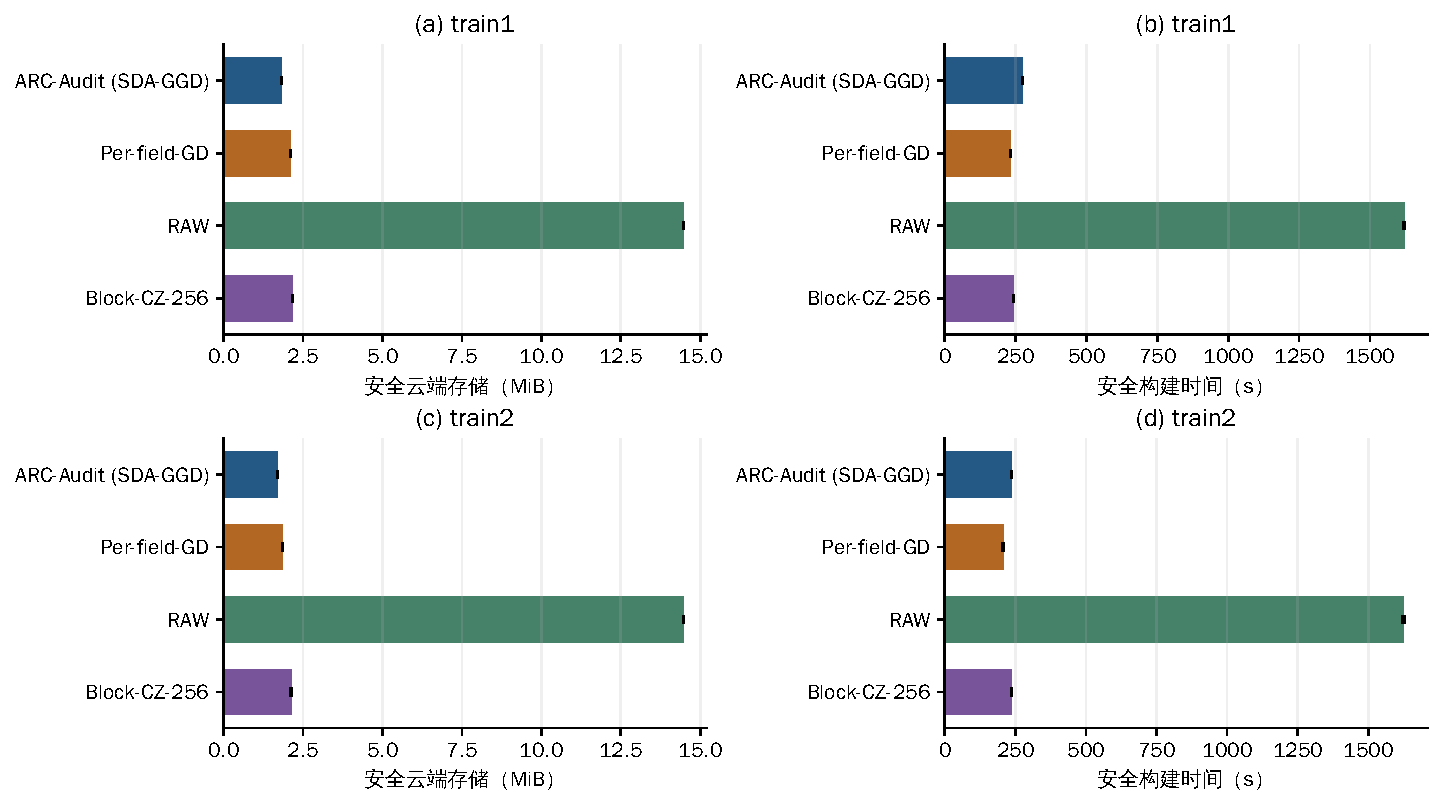
\includegraphics[width=\textwidth]{figures/cn/c1.pdf}
\caption{ARC-Audit（SDA-GGD）与编码基线的存储和构建成本（RQ1）。}
\label{fig:key-c1}\end{figure*}
\begin{figure*}[t]\centering
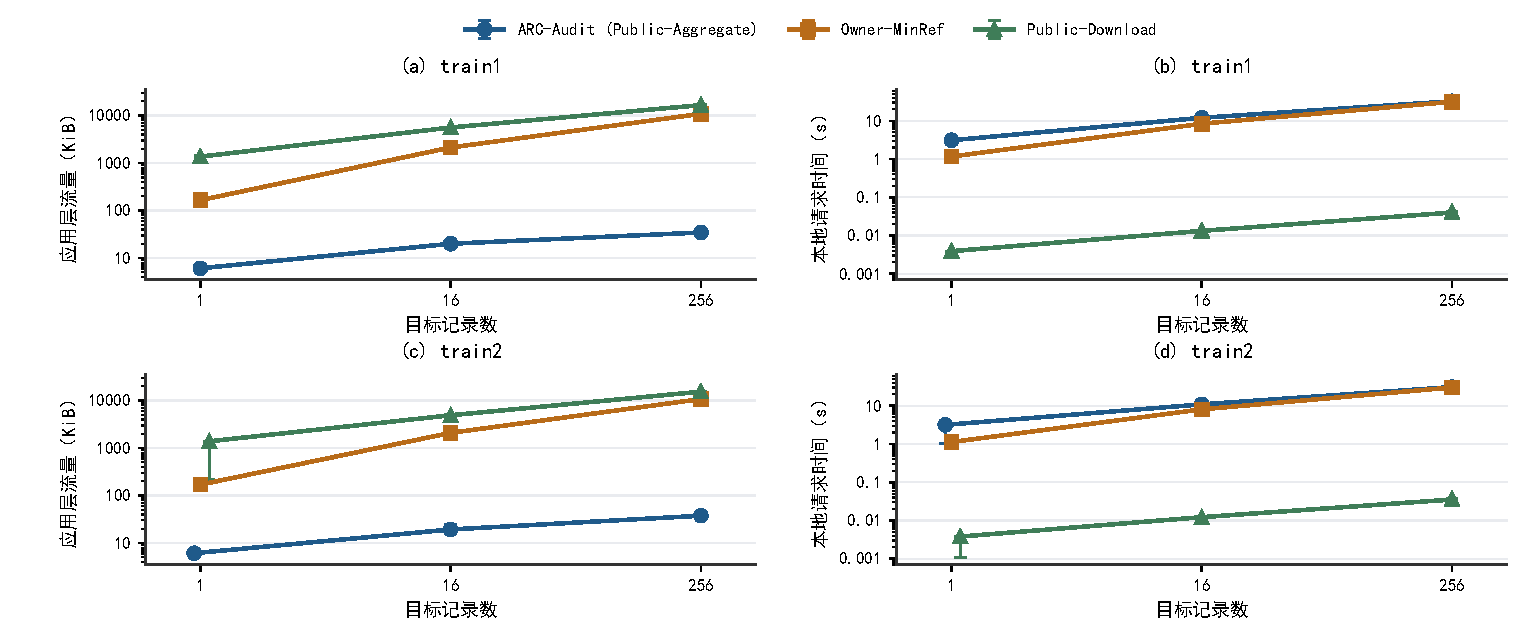
\includegraphics[width=\textwidth]{figures/cn/c2.pdf}
\caption{复用上下文时各接口的每请求应用层流量和本地处理时间（RQ2）。应用层流量包括声明、挑战、可能的第一阶段材料及最终响应；文中所报临界带宽采用简单串行传输估算。}
\label{fig:key-c2}\end{figure*}
\begin{figure*}[t]\centering
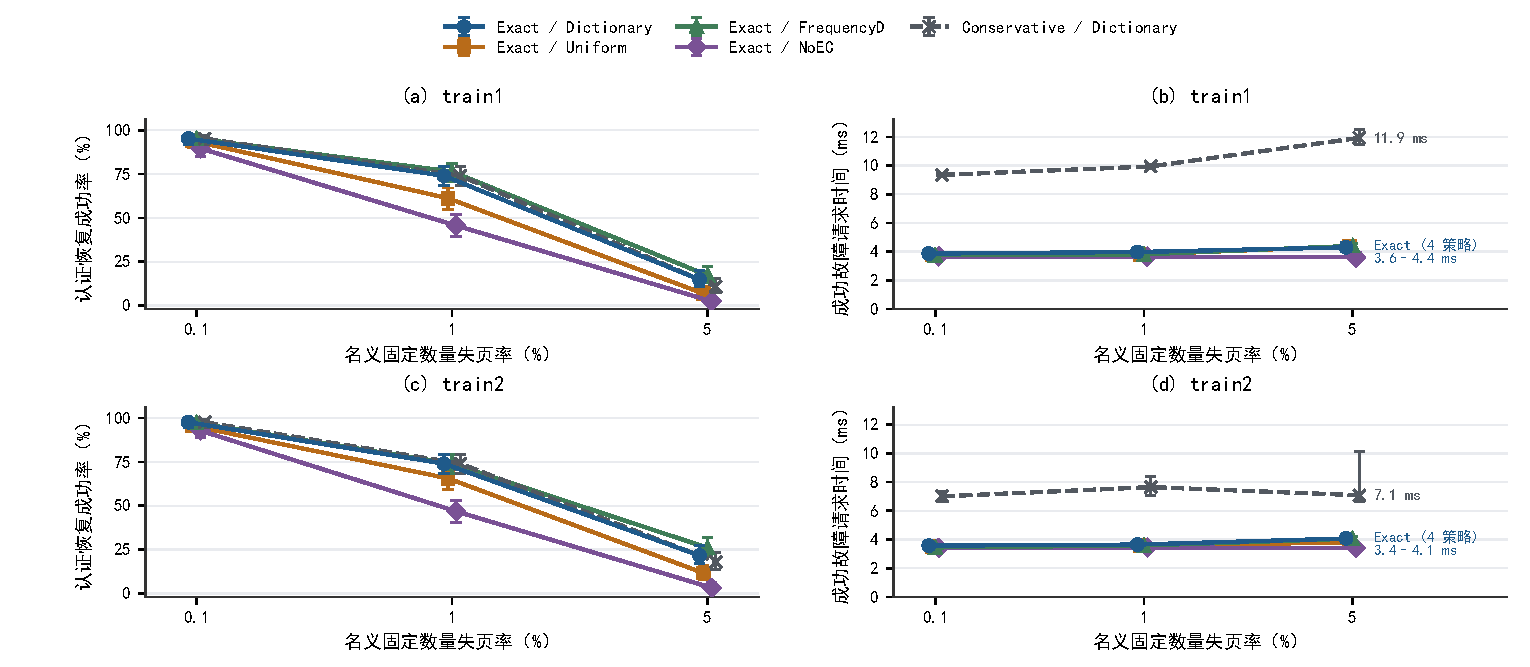
\includegraphics[width=\textwidth]{figures/cn/c3.pdf}
\caption{擦除条件下的认证恢复表现（RQ3）。图例中的 Exact / Dictionary 为精确恢复与字典页优先保护的组合。}
\label{fig:key-c3}\end{figure*}

\subsection{实验设置}
\subsubsection{数据与实现}
本文在 HAI 21.03 工业控制数据集~\cite{Shin2021HAI}~的 \texttt{train1} 与 \texttt{train2} 数据段上评估 ARC-Audit，两者分别包含 216,001 与 226,801 条记录。每条记录含 84 列，包括时间列、79 个过程字段和 4 个攻击指示字段（其中 3 个过程级指示字段独立编码，1 个综合指示字段由前三者导出）。数据导入时采用精确十进制规范化以保留过程值。每次恢复操作完成后，独立评分器以规范化源记录校验 $\widehat r_i=r_i$，该校验独立于客户端的认证与完整解码检查。

RQ1 编码评估对 \texttt{train1} 和 \texttt{train2} 各选取一个含 21,600 条记录的六小时窗口，起点分别为 2020 年 7 月 11 日和 8 月 1 日 00:00。RQ2 审计与 RQ3 恢复评估使用完整数据段：\texttt{train1} 划分为 3 个日批次（依次包含 86,400、86,400 和 43,201 条记录），\texttt{train2} 划分为 4 个日批次（依次包含 7,200、86,400、86,400 和 46,801 条记录）。各批次独立完成配置与加密封装。由于两个数据段均来自同一 HAI 部署，下文成对数值均按 \texttt{train1} 与 \texttt{train2} 顺序给出。

原型系统基于 Python 3.10.12 实现，依赖 NumPy 2.2.6、cryptography 50.0.1 和 py-ecc 8.0.0，集成了 AES-256-GCM、Ed25519、基于 BLS12-381 的整页审计认证器与密文 RS$(10,8)$。同一主机上，编码实验（RQ1）绑定 CPU 2，全量工作负载实验（RQ2 与 RQ3）绑定 CPU 4。输入准备与独立评分不计入构建和请求耗时。请求计时从已初始化的可复用批次上下文中的依赖规划开始，辅助保护上下文亦在恢复计时前完成初始化。

\begin{table}[t]\centering\small
\caption{评估工作负载}\label{tab:scope}
\setlength{\tabcolsep}{4pt}
\begin{tabular}{@{}l>{\raggedright\arraybackslash}p{.25\columnwidth}>{\raggedright\arraybackslash}p{.41\columnwidth}@{}}\toprule
评估范围 & 各数据段记录数 & 对照与观测规模\\\midrule
RQ1（编码） & 21,600 / 21,600 & 4 种方法，各 2 次构建（16 次观测）\\
RQ2（审计） & 216,001 / 226,801 & 3 个目标规模、3 个案例、3 种接口（54 次请求）\\
RQ3（恢复） & 216,001 / 226,801 & 5 个布局、3 个丢失率、50 个案例、8 组对照（12,000 个故障结果）\\
RQ3（无故障） & 同 RQ3 & 30 个案例、1 个布局、8 组对照（480 个结果）\\\bottomrule
\end{tabular}\end{table}

\subsubsection{对照与指标}
针对 RQ1，本文将 ARC-Audit 的 SDA-GGD 编码器与 Per-field-GD、RAW 规范化编码及 Block-CZ-256 进行比较。Block-CZ-256 以 256 条记录为一块序列化非常量字段，再用 Zstd 级别 3 将各块压缩为独立帧。Per-field-GD 对各非常量字段独立应用 GD，以隔离跨字段分组的影响；RAW 与 Block-CZ-256 分别作为未压缩与常规压缩基线。四种表示采用相同的加密认证封装与核算口径。安全云端字节计入密文、审计标签和签名公开清单，所有者侧共享基字节与全部私有磁盘状态则单独报告。构建耗时涵盖规范化输入后的配置、编码和完整加密认证封装。

候选合并排序采用 $\min(50{,}000,n)$ 行样本，因而在 21,600 行的 RQ1 窗口上覆盖全窗；该设置以全窗排序和全量输入成本确认评估分组。实验取 $\rho=1$，使所有测试前缀均可行。每种方法在各窗口上分别以种子 41001 和 41002 构建两次，图表报告中位数及观测范围。

针对 RQ2，本文在目标数 $r\in\{1,16,256\}$ 上分离依赖发现与证明响应格式的影响，每种数据段与目标规模组合测试 3 个目标集合。ARC-Audit 的 Public-Aggregate 接口选取公开闭包；Owner-MinRef-Aggregate（下文及图表中简称为 Owner-MinRef）先认证并解密引用材料以定位精确依赖；Public-Download 则下载公开闭包密文供哈希验证。两个公开接口均不持有解密密钥，而 Owner-MinRef 持有授权解密能力。比较 Public-Aggregate 与 Public-Download 可在相同公开权限下隔离响应格式差异，比较 Public-Aggregate 与 Owner-MinRef 则对比不同访问权限下的依赖规划开销。

同一案例中三种接口测试相同的目标集合，跨批次目标分别由对应批次上下文处理。应用层流量计入声明、挑战、第一阶段引用材料与响应。本地请求时间涵盖依赖规划和接口执行（初始化耗时另行报告），时间轴反映本地计算而非网络传输。图中各数据点给出 3 个匹配目标集合的中位数与最小--最大范围。

针对 RQ3，本文在 Dictionary、Uniform、FrequencyD 与 NoEC 四种保护配置下交叉评估 Exact 与 Conservative 两种依赖选择策略。固定 Exact 可隔离保护位置分配的影响，固定同一保护布局可隔离依赖选择的影响，NoEC 则提供零冗余基线。

所有受保护配置采用相同的 RS$(10,8)$ 编码、相同的准入条带数，以及包含校验分片和签名辅助保护状态的每批次 10\% 密文字节预算。FrequencyD 按各批次前 $\min(4,096,\max(1,\lfloor n/5\rfloor))$ 条记录的依赖频次排序，所有 RQ3 恢复目标均从参考范围之外抽取。因此，7,200 条记录的批次使用 1,440 条参考记录，其余六个批次各使用 4,096 条。独立评分器仅在服务计时结束后读取源记录，恢复流程完全通过云端获取接口与已验证修复获取内容。

\subsubsection{故障与统计}
针对每个数据段，RQ3 采用种子 41001--41005 生成五个保护布局，在名义丢失率 $\alpha\in\{0.001,0.01,0.05\}$ 下为每个布局与丢失率组合测试 50 个单记录恢复案例。每个案例选定一条目标记录，并在整段原始页与已部署校验槽位的并集中无放回抽取固定数量的擦除位置。故障总体规模在 \texttt{train1} 上为 $N_{\mathrm{fault}}=5,000$、在 \texttt{train2} 上为 $4,765$，对应 $\lceil\alpha N_{\mathrm{fault}}\rceil$ 擦除数在 \texttt{train1} 上为 5、50 和 250，在 \texttt{train2} 上为 5、48 和 239。每条目标仅访问其所属批次的对象。所有对照共享相同的目标与槽位丢失掩码（NoEC 仅承受对应的原始页丢失），并在各案例间轮换策略执行顺序。

每个故障成功率数据点汇总全部 250 次结果，并报告以五个测试布局为条件的逐点 95\% Wilson 置信区间。恢复耗时中位数仅在成功故障请求上计算；由于不同对照可能在不同的目标子集上成功，解释耗时时应结合成功率一并考量。无故障恢复在单个布局上对每组数据段与对照各测 30 个案例，共完成 480 次完整记录核验。

\subsection{RQ1：存储与安全构建}
跨字段分组相较所有基线进一步压缩了安全云端存储，同时将部分编码计算转移至所有者端。如图~\ref{fig:key-c1}~所示，ARC-Audit（SDA-GGD）在 \texttt{train1} 与 \texttt{train2} 上的安全云端存储分别为 1,903,138 B 与 1,770,118 B，低于 Per-field-GD 的 2,198,812 B 与 1,938,839 B，云端存储分别降低 13.45\% 和 8.70\%。Block-CZ-256 分别占用 2,278,001 B 与 2,227,359 B，RAW 在每个窗口均占用 14.463 MiB。全部 16 次构建均通过规范化解码检查。

由于合并候选需在全量输入上重新配置，分组增加了总构建耗时，尽管输出页数减少使后续标签生成有所加快。完整安全构建时间中位数由 Per-field-GD 的 231.521 s 与 206.163 s 增至 SDA-GGD 的 274.356 s 与 235.621 s，在 \texttt{train1} 和 \texttt{train2} 上分别增加 18.50\% 和 14.29\%。具体而言，SDA-GGD 在编解码阶段耗时 73.66 s 与 47.63 s（Per-field-GD 分别为 1.00 s 与 0.83 s），而标签生成耗时从 230.25 s 与 205.05 s 降至 200.42 s 与 187.72 s。由于两个 21,600 条记录的窗口均采用全窗排序，上述耗时刻画了全量确认分组流程的开销，更大规模批次上抽样排序的成本与候选覆盖率仍有待测量。

云端存储节省也伴随着更大的所有者侧私有状态（表~\ref{tab:state}）。在 \texttt{train1} 与 \texttt{train2} 上，SDA-GGD 保留的私有状态总量为 335,884 B 与 215,702 B（含共享基内容 303,595 B 与 184,687 B），而 Per-field-GD 的私有状态总量为 245,064 B 与 209,287 B（含共享基 208,267 B 与 174,552 B）。

\begin{table}[t]\centering\small
\caption{云端存储与所有者侧状态（RQ1）}\label{tab:state}
\setlength{\tabcolsep}{4pt}
\begin{tabular}{@{}lrrrr@{}}\toprule
& \multicolumn{2}{c}{云端（MiB）} & \multicolumn{2}{c}{所有者（KiB）}\\
方法 & train1 & train2 & train1 & train2\\\midrule
ARC-Audit（SDA-GGD） & 1.815 & 1.688 & 328.012 & 210.646\\
Per-field-GD & 2.097 & 1.849 & 239.320 & 204.382\\
RAW & 14.463 & 14.463 & 0.227 & 0.227\\
Block-CZ-256 & 2.172 & 2.124 & 0.234 & 0.234\\
\bottomrule\end{tabular}
\tabnote{每窗口两次构建的中位数。所有者状态包含共享基目录与私有编码／密钥文件。保护开销另行核算。}
\end{table}

\subsection{RQ2：公开审计的通信与计算}
\emph{聚合证明与密文下载。}在相同公开闭包上，证明聚合以本地密码学验证为代价将应用层流量降低了两个数量级以上（图~\ref{fig:key-c2}）。在 $r=256$ 时，Public-Aggregate 在 \texttt{train1} 与 \texttt{train2} 上分别传输 35,405 B 与 38,524 B，本地处理耗时为 32.532 s 与 30.908 s；相比之下，Public-Download 传输 17,041,940 B 与 15,754,868 B，本地摘要核验仅需 0.0400 s 与 0.0354 s。以节省的比特数除以额外本地处理时间，可估得简单串行传输的临界带宽为 4.19 Mbit/s 与 4.07 Mbit/s（未计入初始化、网络往返及传输与计算重叠）。

\emph{公开规划与授权引用解析。}公开闭包规划省去了第一阶段引用传输，同时在较大目标规模下保持与授权引用解析相近的本地运行时间。Owner-MinRef 先认证解密引用以缩减最终字典覆盖范围，因而引入额外的引用流量。在 $r=256$ 时，Owner-MinRef 传输 11,163,473 B 与 11,010,612 B，本地耗时 31.532 s 与 30.148 s。相较 Owner-MinRef，Public-Aggregate 将应用层流量减少 99.68\% 与 99.65\%（按观测中位数计算），本地处理时间仅增加 3.17\% 与 2.52\%。

在较小目标规模下，由于单条记录涉及的字典页较少，引用解析能省去更多本地配对运算，但仍需承担可观的引用传输。当 $r=1$ 时，Public-Aggregate 传输 6,237 B 与 6,254 B、本地耗时 3.106 s 与 3.169 s，而 Owner-MinRef 传输 169,601 B 与 173,696 B、本地耗时 1.164 s 与 1.126 s。随着 $r$ 增大，跨目标页重叠与引用并集缩小了这一耗时差距：在 $r=16$ 时，Public-Aggregate 传输 20,512 B 与 19,742 B、本地耗时 12.015 s 与 10.902 s，Owner-MinRef 则传输 2,179,425 B 与 2,138,835 B、本地耗时 8.404 s 与 8.066 s。

\emph{流量构成与上下文复用。}在 $r=256$ 时，引用材料占 Owner-MinRef 流量的绝大部分，其第一阶段传输量中位数达 11,128,596 B 与 10,972,500 B，而两个公开接口均免除了该部分传输。两个聚合接口每批次固定返回 4,310 B 的证明（在三个 \texttt{train1} 批次上合计 12,930 B，在四个 \texttt{train2} 批次上合计 17,240 B），其余流量由声明与挑战构成。上述请求耗时基于跨请求复用的已初始化批次上下文；$r=1$ 时冷启动初始化中位耗时为 8.101 s 与 7.805 s，$r=256$ 时冷启动需传输 1,678,681 B 与 1,623,188 B 并耗时 20.816 s 与 21.168 s。全部 54 次诚实请求均通过各自接口的验证。

\emph{机制对照。}表~\ref{tab:c2-mechanisms}~在 7 月 11 日 \texttt{train1} 批次与 7 月 31 日 \texttt{train2} 批次的两个 16 目标请求上，分别隔离了读取复用、证明聚合与数据表示的贡献。并集规划与带请求内缓存的逐记录遍历均对每个选中对象只读取一次；在固定页集合与挑战系数下，证明聚合大幅削减了证明字节与验证时间。两个批次中被篡改末字节的密文测试均被拒绝。在保持目标、并集规划器与聚合后端一致时，SDA-GGD 选中的页数少于 Per-field-GD，从而在两次请求中均降低了服务端读取量与本地处理时间，且两种表示每批次仍返回 4,310 B 证明。

\begin{table}[t]\centering\small
\caption{两个 16 目标请求的审计机制对照（RQ2）}
\label{tab:c2-mechanisms}
\setlength{\tabcolsep}{3.2pt}
\begin{tabular}{@{}lrrrr@{}}\toprule
 & \multicolumn{2}{c}{train1} & \multicolumn{2}{c}{train2}\\
\cmidrule(lr){2-3}\cmidrule(l){4-5}
读取方式 & 次数 & 字节 & 次数 & 字节\\\midrule
逐记录 & 5,643 & 23,113,728 & 892 & 3,651,221\\
逐记录加缓存 & 805 & 3,297,280 & 125 & 509,589\\
并集 & 805 & 3,297,280 & 125 & 509,589\\\midrule
证明格式 & 字节 & 验证（s） & 字节 & 验证（s）\\\midrule
逐页 & 3,475,990 & 472.659 & 539,750 & 73.646\\
聚合 & 4,310 & 3.477 & 4,310 & 1.074\\\midrule
数据表示 & 页数 & 本地（s） & 页数 & 本地（s）\\\midrule
Per-field-GD & 883 & 7.023 & 143 & 1.683\\
SDA-GGD & 805 & 6.437 & 125 & 1.489\\\bottomrule
\end{tabular}
\tabnote{不带缓存的逐记录遍历按实际读取次数计数。表示布局对照中，SDA-GGD 的读量见并集行，Per-field-GD 在 train1 上读取 3,616,768 B，在 train2 上读取 585,227 B。}
\end{table}

\subsection{RQ3：认证恢复与保护分配}
\emph{保护位置。}在相同存储预算下，优先保护字典页始终优于均匀冗余分配（图~\ref{fig:key-c3}）。固定 Exact 恢复策略并在 1\% 名义丢失率下，Dictionary 在两个数据段均于 250 次中恢复 185 条记录（74.0\%），而 Uniform 在 \texttt{train1} 上恢复 153 条（61.2\%）、在 \texttt{train2} 上恢复 164 条（65.6\%），对应 12.8 与 8.4 个百分点的优势；无冗余的 NoEC 仅恢复 114 条（45.6\%）与 117 条（46.8\%）。在 0.1\% 丢失率下，Dictionary 的恢复率达到 95.2\% 与 97.6\%，高于 Uniform 的 94.0\% 与 95.6\%。

\emph{基于频率的分配。}在 5\% 名义丢失率下，按参考工作负载依赖频次排序（FrequencyD）相比按对象类型排序（Dictionary）具有一定额外优势。在 5\% 丢失率与 Exact 恢复下，FrequencyD 在 \texttt{train1} 上恢复 250 次中的 43 条记录（17.2\%）、在 \texttt{train2} 上恢复 65 条（26.0\%），而 Dictionary 分别为 14.8\% 与 21.6\%。跨越五个测试布局的配对差异在 \texttt{train1} 上为 $-2$ 至 $+8$ 个百分点、在 \texttt{train2} 上为 $0$ 至 $+12$ 个百分点（表~\ref{tab:paired-layouts}）；在编码、条带数与预算固定时，调整排序会同时改变受保护页集合与条带成员划分。在 1\% 丢失率下，FrequencyD 分别恢复 191 条与 185 条（Dictionary 两段均为 185 条）；在 0.1\% 丢失率下，两者在 \texttt{train1} 上持平，Dictionary 在 \texttt{train2} 上略高。

\emph{依赖策略。}在 5\% 名义擦除率且固定 Dictionary 保护时，将取页收窄至精确依赖使部分在未使用字典页丢失情况下原本失败的请求得以完成。Exact 恢复了 Conservative 成功的所有记录，并在 \texttt{train1} 上额外恢复 10 条、在 \texttt{train2} 上额外恢复 9 条，将完整记录恢复数从 Conservative 的 250 次中 27 条（10.8\%）与 45 条（18.0\%）提升至 Exact 的 37 条（14.8\%）与 54 条（21.6\%）。上述 4.0 与 3.6 个百分点的提升在 5\% 擦除率与 10\% 冗余上限下仍对应 85.2\% 与 78.4\% 的失败率。在所有新增成功案例中，实际依赖页均已取得或修复，仅未被引用的字典页不可用。在 0.1\% 与 1\% 名义擦除率下，两种策略成功恢复的是同一批请求。

\begin{table}[t]
\centering\small
\caption{5\% 擦除率下的配对恢复结果（RQ3）}
\label{tab:paired-layouts}
\setlength{\tabcolsep}{3pt}
\begin{tabular}{@{}llrrrrr@{}}
\toprule
数据段 & 对照 & 41001 & 41002 & 41003 & 41004 & 41005 \\
\midrule
train1 & F/D & 0/1 & 2/2 & 5/1 & 3/1 & 4/3 \\
       & D/U & 9/0 & 3/1 & 3/3 & 2/0 & 8/1 \\
       & E/C & 3/0 & 1/0 & 1/0 & 2/0 & 3/0 \\
\midrule
train2 & F/D & 2/1 & 4/0 & 7/1 & 2/2 & 2/2 \\
       & D/U & 4/0 & 7/0 & 4/2 & 8/2 & 7/1 \\
       & E/C & 1/0 & 2/0 & 2/0 & 2/0 & 2/0 \\
\bottomrule
\end{tabular}
\tabnote{列为布局种子。每格表示 50 个配对案例中仅由前一配置／后一配置成功恢复的数量。F、D、U 分别表示 Exact 下的 FrequencyD、Dictionary 和 Uniform。E/C 在固定 Dictionary 保护布局下比较 Exact 与 Conservative。}
\end{table}

\emph{恢复时间。}Exact 恢复由于获取并解密更少的认证字节，还带来了更低的延迟。在无故障 Dictionary 实验中，两种策略恢复相同目标，Exact 在 \texttt{train1} 与 \texttt{train2} 上的中位耗时分别为 3.693 ms 与 3.507 ms，而 Conservative 分别为 8.991 ms 与 7.205 ms。在 5\% 名义丢失率且固定 Dictionary 保护时，Exact 成功请求的中位耗时为 4.298 ms 与 4.074 ms（Conservative 为 11.933 ms 与 7.079 ms，均含取页与必要的 RS 修复），失败请求则分别在 0.414 ms 与 0.461 ms 内中止（Conservative 为 5.810 ms 与 3.892 ms）。由于故障条件下两种策略成功的请求集合不同，成功请求中位数各自刻画其自身成功子集上的完成时间。

综上，保护分配决定哪些对象获得冗余，依赖选择决定请求必须取得哪些对象。在固定保护布局与验证规则下，缩减所需页集合因此能够让更多请求在所测 HAI 工作负载与擦除设置下完成恢复。

\subsection{实验产物}
归档评估包 \texttt{dual\_hai\_20261008\_v3} 完整保留了精简配置的编码实验（RQ1）以及全量工作负载下的审计与恢复实验（RQ2 与 RQ3），其中包含逐案观测、机制对照、原型源码快照以及记录输入与源码哈希的配置清单。自动核验脚本可依据归档清单复算全部报告的统计指标，并校验每批次序列化保护文件是否满足存储上限。

\section{结论}
ARC-Audit 利用单一认证布局协调共享压缩 IIoT 记录的公开审计与授权恢复。无需解密密钥时，公开验证者构造覆盖目标记录全部潜在字典依赖的充分闭包，并将其绑定至新鲜聚合挑战；持有解密密钥时，授权恢复者先认证引用以将检索缩窄至精确依赖，同时对修复页与直接获取页施以相同的完整性校验。

在两个 HAI 数据段上，ARC-Audit 的分组表示相较按字段独立 GD 分别降低了 13.45\% 与 8.70\% 的安全云端存储开销，代价是更长的构建时间；在相同闭包上，公开聚合显著削减了应用层流量并伴随更高的本地计算。在 5\% 名义擦除率与固定字典页优先保护条件下，每当未引用字典页丢失时，精确依赖解析使完整记录恢复率相较保守闭包恢复分别提高 4.0 与 3.6 个百分点。未来工作将把认证依赖映射扩展至跨批次共享字典并量化页复用对索引与清单更新的影响，评估相关故障与整批不可用下的恢复率及修复读放大，并在更多工业物联网数据集上检验上述策略。

\IEEEtriggeratref{24}
\bibliographystyle{IEEEtran}
\bibliography{IEEEabrv,bstcontrol,references}
\end{document}
